\section{Auswertung}
\label{sec:Auswertung}

\subsection{Daten der verwendeten Helmholtzspulenpaare}

Die verwendeten Spulen haben folgende Abmessungen, wobei der Radius mit $R$ und die Windungszahl mit $N$ gegeben ist:

\begin{align*}
  R_\text{Horizontalfeldspule} &= \SI{15.79}{\centi\meter}\,,\\
  R_\text{Sweepfeldspule} &= \SI{16.39}{\centi\meter}\,,\\
  R_\text{Vertikalfeldspule} &= \SI{11.735}{\centi\meter}\,,\\
  N_\text{Horizontalfeldspule} &= \num{154}\,,\\
  N_\text{Sweepfeldspule} &= \num{11}\,,\\
  N_\text{Vertikalfeldspule} &= \num{20}\,.\\  
\end{align*}

\subsection{Korrektur des vertikalen Erdmagnetfeldes}

Zur Korrektur des vertikalen Erdmagnetfeldes wird der Aufbau entsprechend \label{sec:Durchführung} ausgerichtet und das Feld der Vertikalfeldspule auf $T_\text{vert} = \SI{0.229}{\ampere}$
eingestellt. Gemäß \eqref{eqn:helm} kompensiert das Feld der Vertikalfeldspule also ein vertikales Erdmagnetfeld von 

\begin{equation*}
  B_\text{vert} = \SI{35.09}{\micro\tesla}\,.
\end{equation*}

\subsection{Vermessen des Magnetfeldes in Abhängigkeit von der Resonanzfrequenz}

Die im Versuch gemessenen Ströme in Abhängigkeit von der Frequenz des Wechselfeldes sind in Tabelle \ref{tab:mess1} angegeben.

\begin{table}
  \centering
  \caption{Die für die Horiuontalfeld- und Sweepspulen gemessenen Ströme $I_\text{H}$ und $I_\text{S}$ für die Resonanzen 1 und 2 und daraus errechneten Magnetfeldstärken $B$ in Abhängigkeit der angelegten Frequenz $f$.}
  \label{tab:mess1}
  \sisetup{table-format=2.1}
  \begin{tabular}{c c c c c c c}
  \toprule
  $f \,/\, \si{\kilo\hertz}$ & $I_\text{H1} \,/\, \si{\ampere}$ & $I_\text{S1} \,/\, \si{\ampere}$
  & $B_\text{hor,1} \,/\, \si{\micro\tesla}$ & $I_\text{H2} \,/\, \si{\ampere}$ & $I_\text{S2} \,/\, \si{\ampere}$
  & $B_\text{hor,2} \,/\, \si{\micro\tesla}$\\
  \midrule 
       100& 0    & 0,043&  37,7& 0    & 0,051&  44,7\\
       200& 0    & 0,060&  52,7& 0    & 0,077&  67,5\\
       300& 0    & 0,077&  67,5& 0    & 0,102&  89,5\\
       400& 0    & 0,094&  82,4& 0    & 0,127& 111,4\\
       500& 0    & 0,110&  96,5& 0    & 0,152& 133,3\\
       600& 0    & 0,127& 111,4& 0,315& 0,153& 153,2\\
       700& 0    & 0,144& 126,3& 0,456& 0,168& 174,8\\
       800& 0,075& 0,153& 138,7& 0,945& 0,157& 194,7\\
       900& 1,245& 0,086& 150,6& 1,245& 0,162& 217,2\\
      1000& 1,818& 0,060& 162,3& 1,818& 0,144& 236,0\\
  \bottomrule
  \end{tabular}
\end{table}

Hierbei bezeichnet $I_\text{H}$, $I_\text{S}$ und $B_\text{hor}$ die für die jeweiligen Resonanzen eingestellten Stromstärken an Horizontal- und 
Sweepspule, sowie das daraus resultierende gesamte horizontale Magnetfeld. Dieses ist durch die lineare Superposition der einzelnen Magnetfelder
errechenbar.\\
Werden Frequenzen und horizontale Magnetfeldstärke gegeneinander aufgetragen und eine Regressionsgerade durch die Messwerte gelegt, ergeben 
sich Abbildung \ref{fig:plot1} und Abbildung \ref{fig:plot2}.

\begin{figure}
  \centering
  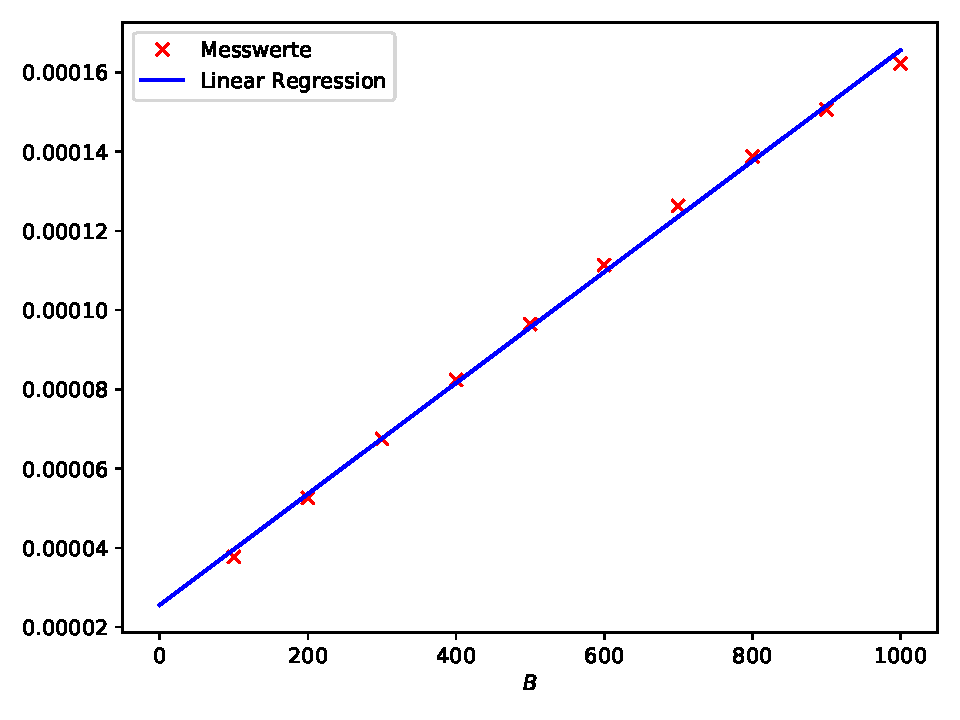
\includegraphics[scale=0.6]{content/plot1.pdf}
  \caption{Lineare Regression der Magnetfeldstärken in Abhängigkeit von der Resonanzfrequenz für Isotop 1.}
  \label{fig:plot1}
\end{figure}

\begin{figure}
  \centering
  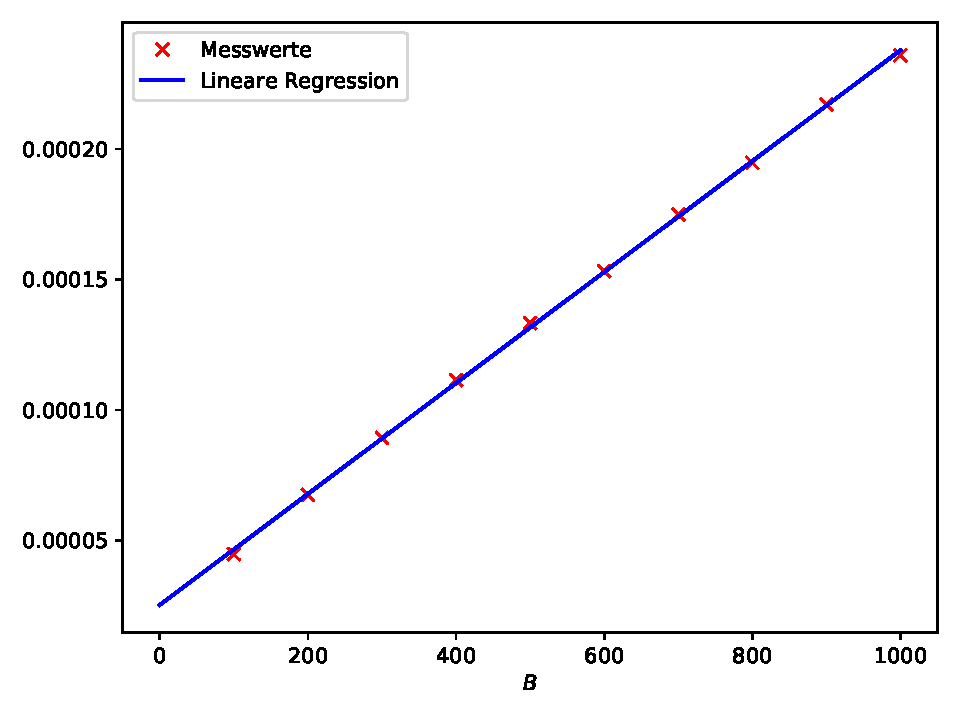
\includegraphics[scale=0.6]{content/plot2.pdf}
  \caption{Lineare Regression der Magnetfeldstärken in Abhängigkeit von der Resonanzfrequenz für Isotop 2.}
  \label{fig:plot2}
\end{figure}

Die Ausgleichsrechnungen werden mit der Funktion

\begin{equation*}
  f = a\cdot B_\text{hor} + b
\end{equation*}

durchgeführt. Es ergeben sich für $b$ die Werte

\begin{align*}
  b_1 &= \num{25.6\pm 1.3}\si{\micro\tesla}\,,\\
  b_2 &= \num{25.4\pm 0.9}\si{\micro\tesla}\,.\\
\end{align*}

Aus diesen Werten wird der Mittelwert zu 

\begin{equation*}
  \bar{b} = \num{25.5\pm 1.2}\si{\micro\tesla}
\end{equation*}

berechnet. Damit wird die Horizontalkomponente des Erdmagnetfeldes abgeschätzt.\\
Aus den Regressionsrechnungen ergeben sich für $a$ die Werte:

\begin{align*}
  a_1 &= \num{140.0\pm 2.1}\si{\micro\tesla\per\mega\hertz}\,,\\
  a_2 &= \num{212.5\pm 1.4}\si{\micro\tesla\per\mega\hertz}\,.\\
\end{align*}

Aus diesen Werten ergibt sich mit 

\begin{equation*}
  g_\text{F} = \frac{h}{a\cdot \mu_\text{B}}
\end{equation*}

der Landefaktor der Isotope zu

\begin{align*}
  g_\text{F1} &= \num{0.519\pm 0.008},\\
  g_\text{F2} &= \num{0.336\pm 0.002}.
\end{align*}

Mit Gleichung \eqref{eqn:lande} und 

\begin{align*}
  g_\text{J} &= \num{2.0023}\,,\\
  J &= \frac{1}{2}\,,\\
  L &= 0\,,\\
  S &= \frac{1}{2}\,,\\
  F &= I +\frac{1}{2}\,,\\
\end{align*}

ergeben sich die Kernspins der Isotope mit 

\begin{equation*}
  I = \frac{1}{2}\left|\frac{g_\text{J}}{g_\text{F}}-1\right|
\end{equation*}

zu 

\begin{align*}
  I_1 &= \num{1.416\pm 0.030}\,,\\
  I_2 &= \num{2.477\pm 0.019}\,.
\end{align*}

\subsection{Bestimmung des Isotopenverhältnisses}

Bei einer RF-Frequenz von $\SI{200}{\kilo\hertz}$ wird das Oszilloskopbild der Resonanzpeaks in Abbildung \ref{fig:iso} aufgenommen.

\begin{figure}
  \centering
  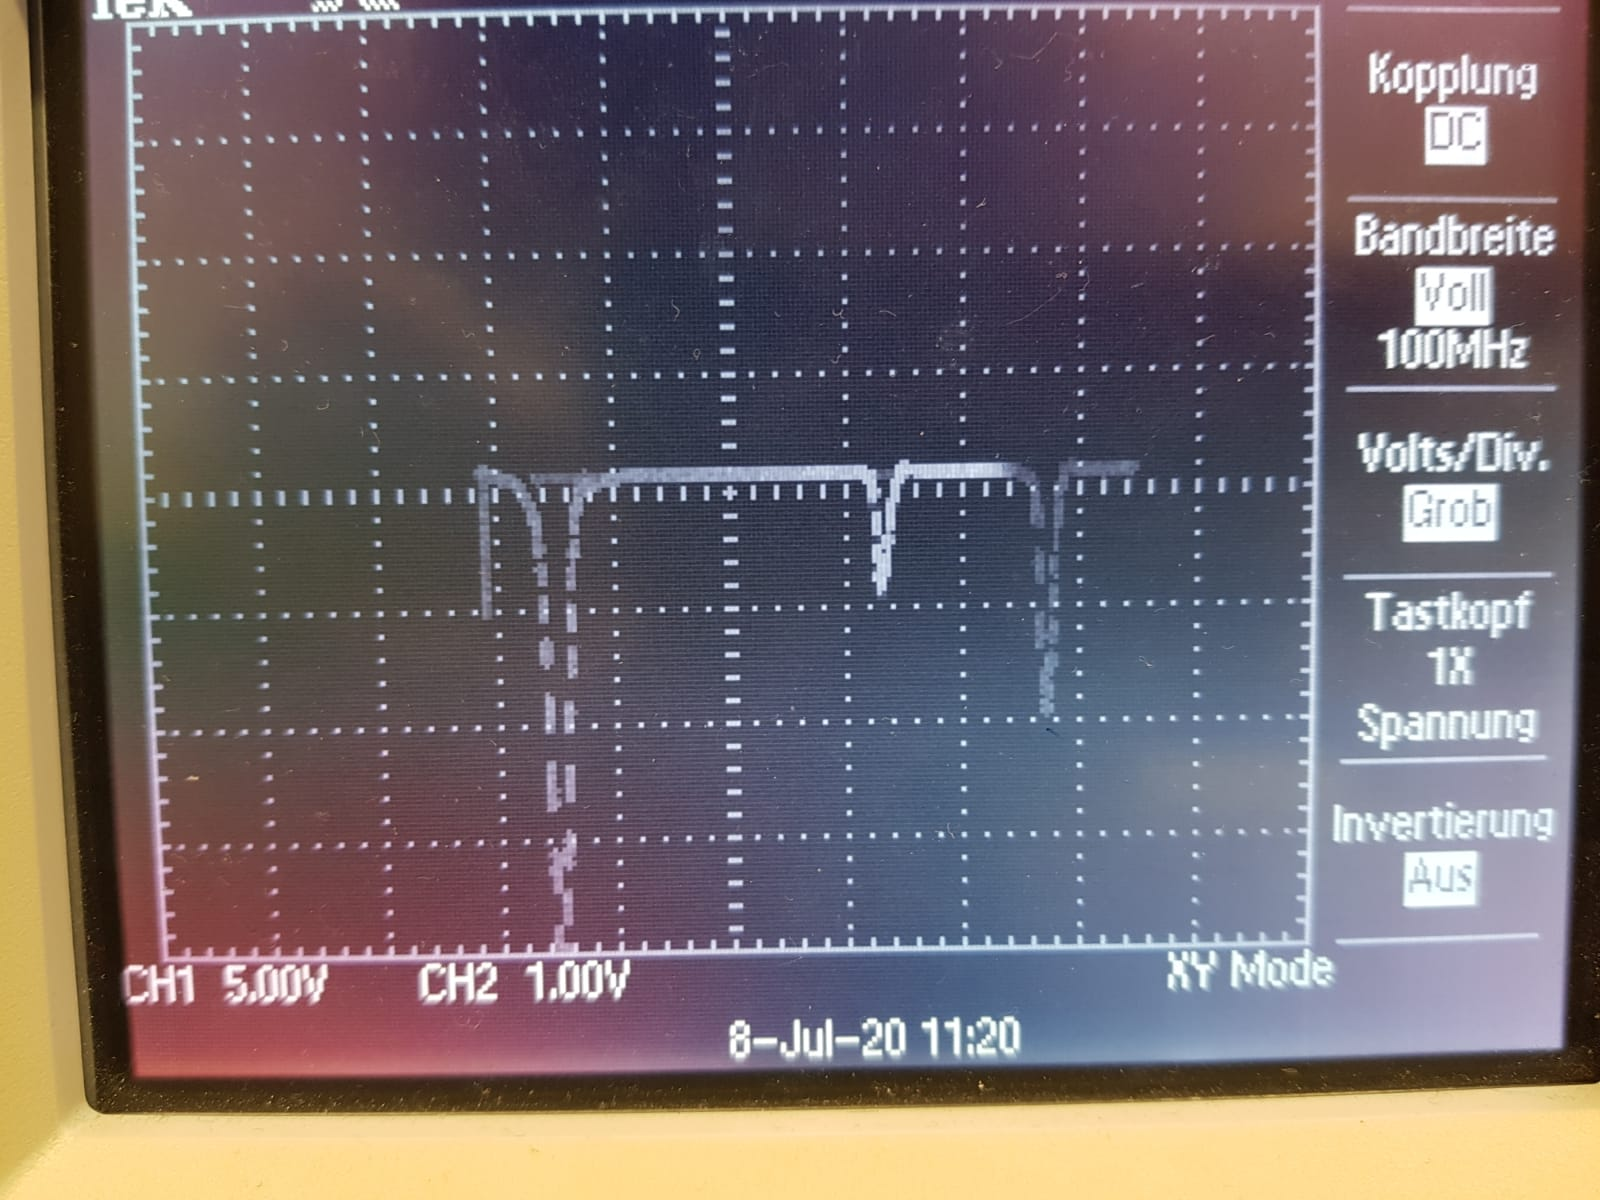
\includegraphics[scale=0.2]{content/iso.jpeg}
  \caption{Oszilloskopbild der Transmissivität in Abhängigkeit vom horizontalen Magnetfeld bei einer RF-Frequenz von $\SI{200}{\kilo\hertz}$.}
  \label{fig:iso}
\end{figure}

Die Höhe der Resonanzpeaks wird wie folgt ermittelt: 

\begin{align*}
  h_1 &= 4 \,\text{Punkte}\,,\\
  h_2 &= 10 \,\text{Punkte}\,.
\end{align*}

Gemäß

\begin{equation*}
  \frac{N_1}{N_2} = \frac{h_1}{h_2}
\end{equation*}

ergibt sich das Isotopenverhältnis zu 

\begin{equation*}
  \frac{N_1}{N_2} = \num{0.4}\,.
\end{equation*}

\subsection{Abschätzung des quadratischen Zeeman-Effekts}

Zunächst wird das erste Isotop betrachtet. Mit

\begin{align*}
  M_\text{F} &= -1\,,\\
  B_\text{max} &= \SI{162.3}{\micro\tesla}\,,\\
  \symup{\Delta}E_\text{Hy} &= \SI{4.53e-24}{\joule}\,,\\
\end{align*}

und \eqref{eqn:quad} kann der maximale quadratische Zeeman-Effekt zu 

\begin{equation*}
  Z_\text{qmax,1} = \num{3.91\pm 0.12e-31}\si{\joule}
\end{equation*}

abgeschätzt werden. Der maximale lineare Zeeman-Effekt beträgt hier mit Gleichung \eqref{eqn:lin}

\begin{equation*}
  Z_\text{lmax,1} = \num{7.68\pm 0.12e-28}\si{\joule}\,.
\end{equation*}

Für Isotop 2 gilt

\begin{align*}
  M_\text{F} &= -2\,,\\
  B_\text{max} &= \SI{236}{\micro\tesla}\,,\\
  \symup{\Delta}E_\text{Hy} &= \SI{2.01e-24}{\joule}\,,\\
\end{align*}

womit der maximale quadratische Zeeman-Effekt zu 

\begin{equation*}
  Z_\text{qmax,2} = \num{1.35\pm 0.02e-54}\si{\joule}
\end{equation*}

abgeschätzt wird. Der maximale lineare Zeeman-Effekt wird hier zu 

\begin{equation*}
  Z_\text{lmax,2} = \num{7.36\pm 0.05e-28}\si{\joule}\,
\end{equation*}

abgeschätzt.